\chapter{SLAM Mapping}\label{chp:slam_mapping}

One of the first challenges in indoor navigation for assistive robots is actually finding where they are. Robot localization is fundamental to not only know where you need to go, but rather find a path there that avoids the obstacles.

Mapping is an essential tool in this matter, and it comprises the areas of \textit{concurrent mapping} and \textit{localization problem}. On themselves, both problems are relatively easy and well understood: mapping an environment knowing the localization and localizing the robot having the map in hands are simple tasks, however the combination of those two problems is hard to solve \cite{thrun2000real}.

Many SLAM (Simultaneous Localization and
Map Building) algorithms emerged to try and solve these problems, using different approaches and range of sensors to do the task. Some even evolved fusing data from different sensors to provide higher precision.

\section{Sensors}

\subsection{Laser Scanners}

The laser scanner is one of the most simple ways to capture data about the environment. They work by sending beams of light in a direction and measuring the time it takes for the light to travel back and forth between the object and the sensor. As you want information to be gathered on more than a single point, the scanner can rotate a mirror or even the whole sensor to gather measurements from all directions, as shown on \prettyref{fig:sick_s300_diagram}. There are two main ways of measuring the object distance: time of flight and Phase-Shift \cite{amann2001laser}.

\begin{figure}
     \centering
     \subfloat[][]{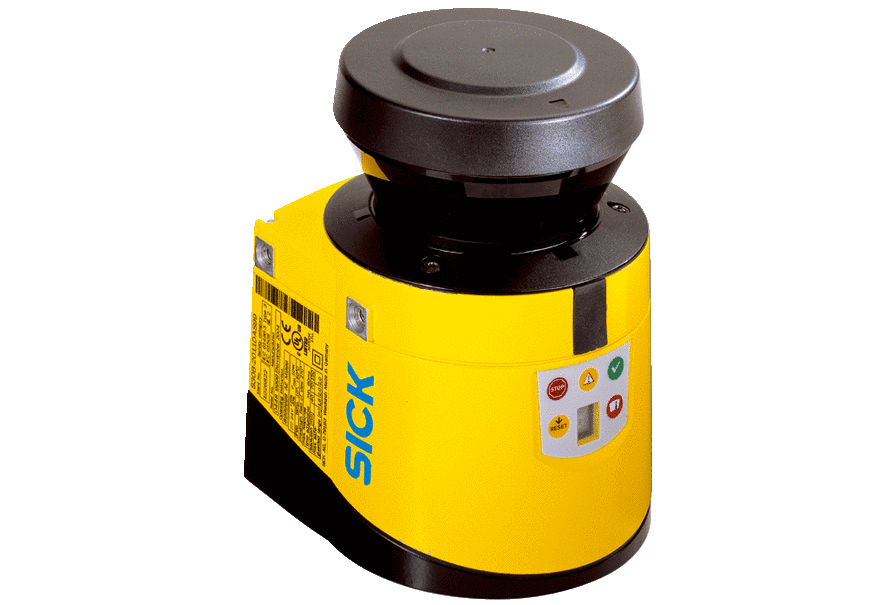
\includegraphics[width=80mm]{sick_s300}}
     \subfloat[][]{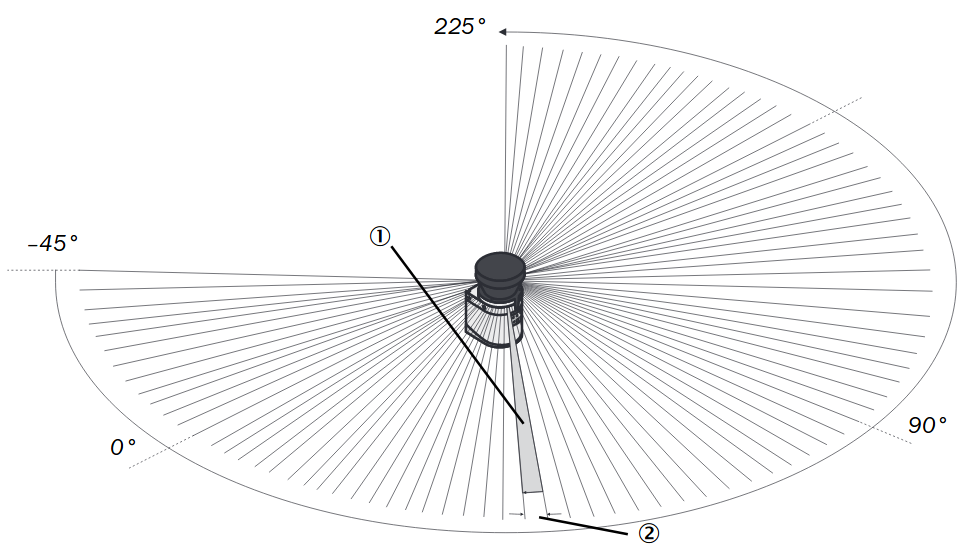
\includegraphics[width=80mm]{sick_s300_diagram}\label{fig:sick_s300_diagram}}
     \caption{SICK S300 Laser Scanner \cite{sicks300}.}
     \label{fig:sick_s300}
\end{figure}

In the time of flight measurement, a stopwatch is started when the beam of light is emitted. Since the speed of light is well known, the calculations are very straight forward, as shown on \prettyref{eq:d}. This form of measurement depends heavily on the quality of construction, as the usual sources of inaccuracy are noise (electronics, radiation in the room), timing (stopwatch precision, pulse detection), and minimal changes in each measurement can lead to big errors in the final result. Averaging and Filtering also take a big role in providing reliable data.

\begin{equation} \label{eq:d}
D = \frac{c \cdot t}{2}
\end{equation}

The second way of calculating the distance is by using phase-shift techniques, assuming there will be a difference in phase between the beam of light emitted and received. This varies according to the frequency and time traveled according to the equation $\phi = \omega \cdot t$, where $\phi$ is the phase-shift, $t$ the time traveled and $\omega$ the angular frequency of the wave. Isolating $t$ and substituting in \prettyref{eq:d}, we can derive the \prettyref{eq:d2} that dictates the distance based on frequency. This technique also requires more complex signal processing structures like a heterodyne for good for measurements.

\begin{equation} \label{eq:d2}
D = \frac{1}{2} \frac{c \cdot \phi}{\omega} = \frac{1}{4 \pi} \frac{c \cdot \phi}{f}
\end{equation}

\subsection{3D cameras}

Even though it is possible to recreate a 3D model of the environment using LIDAR laser scanners, discussed on the last subsection, those sensors coast thousands of dollars and are not very suited for robotics. Fortunately, it is possible to replace those sensors with 3D cameras capable of registering depth based on image processing techniques.

\section{Localizing the robot}

\subsection{Wheel Odometry}

Wheel odometry is one of the most simple ways to determine the position of the robot based on the starting point. Considering a flat surface, simply taking the turns made by each wheel and the steering actions, it is possible to estimate the path the robot took by applying the forward kinematics of the base.

The main disadvantages of wheel odometry are that the robot is limited to flat terrain, and even then slippery and small changes to forward kinematics (i.e. radius of the wheel changes slightly) can accumulate error over time.

\subsection{IMU}

The inertial measurement unit or IMU is an electronic device capable of measuring acceleration. They mostly measure linear and angular acceleration in all the 6 axis. The first 3 axis consist of linear acceleration, when the velocity changes on the X, Y and Z axis. The gyroscopes can also detect changes of angular velocity on the X, Y and Z axis, when the sensor rotates.

This information can be used to build a trajectory by integrating the position twice and adding the starting point:

\begin{equation}
P(t) = P(0) + \int_0^t \int_0^t A(\tau) \ d\tau d\tau
\end{equation}

It is clear that this alone is not a good form of odometry, as it also integrates the error, making the measurement drift from the ground truth as time goes on. This is usually corrected by gathering other forms of data, like GPS or other forms of odometry, so that the error can be reset from time to time.

\section{Building a map}

One of the concerns of mobile robots is how to build a map that is compatible with the environment. While in some applications it is possible to have a pre-compiled map, those can be obsolete when dealing with highly dynamic environments. And even in static environments, there is a need to compensate for faulty or noise sensors, errors in localization, and the pre-compiled maps should be used as complementary information. One of the techniques that emerged to solve these problems, and later was adopted as the core of many SLAM algorithms, is the Occupancy Grid \cite{elfes1989using}.

The Occupancy Grid is form of representing obstacles in 2D or 3D where each cell on the grid stores the probabilistic information of that area. This especially useful because it provides a comprehensive way to fuse sensor data, based on probability, instead of out-of-the-box algorithms that require fine tuning to work.

\begin{figure}[!ht]
    \centering
    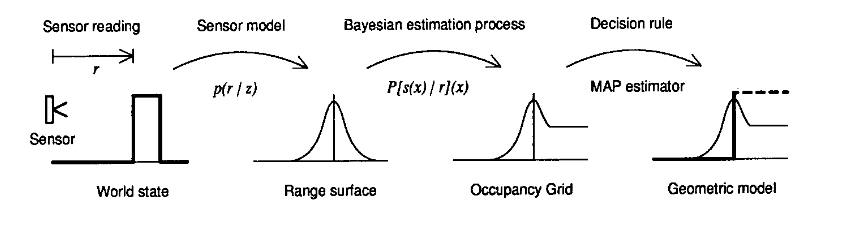
\includegraphics[width=.9\linewidth]{grid_steps}
    \caption{Steps when building an occupancy grid \cite{elfes1989using}.}
    \label{fig:grid_steps}
\end{figure}

According to \prettyref{fig:grid_steps}, the first step when building a sensor grid is to get the sensor reading. The next step is build a sensor model $p(r|z)$. Then, the Bayesian estimation is applied, based on all the observations before and current observations, to update the map. Finally, the world model is obtained using an estimator such as \textit{maximum a posteriori} (MAP).

Naturally, the obstacle cell is labeled as occupied, with probability 1. All the cell until this one are labeled as empty, with probability 0. The unknown cells are labeled with unknown, with probability 0.5.

\begin{figure}[!ht]
    \centering
    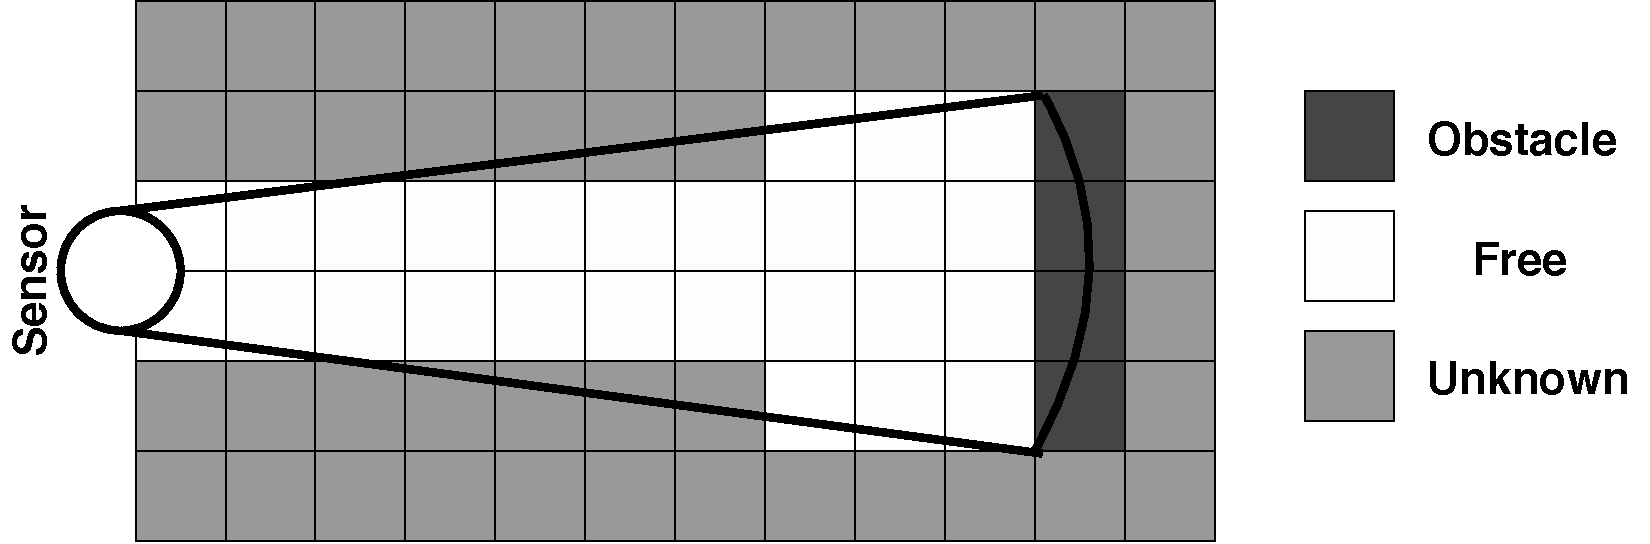
\includegraphics[width=.9\linewidth]{occupancy_grid}
    \caption{Occupancy grid for a single sensor.}
    \label{fig:occupancy_grid}
\end{figure}

The process is iterative and as measurements from different points of view and different sensors grow, the maps become more and more complete, as shown on \prettyref{fig:occupancy_grid_algorithm}.

\begin{figure}[!ht]
    \centering
    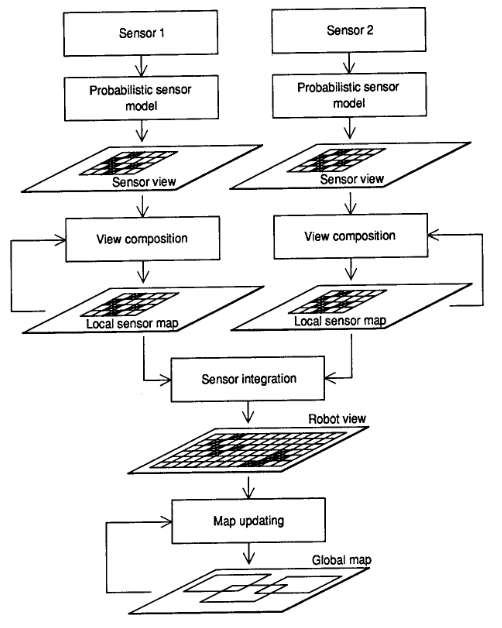
\includegraphics[width=.9\linewidth]{occupancy_grid_algorithm}
    \caption{Occupancy grid algorithm for multiple sensors.}
    \label{fig:occupancy_grid_algorithm}
\end{figure}

\section{SLAM algorithms}

\subsection{Gmapping}

\subsection{Hector}

\subsection{Karto}

\subsection{Frontier Exploration}

\subsection{Cartographer}

\subsection{Comparação}